\documentclass[a4paper, 10pt]{paper}
\usepackage{graphicx}
\usepackage{fullpage}
\usepackage{amsmath}
\usepackage{amssymb}
\usepackage{hyperref}
\usepackage{tcolorbox}
\usepackage{tikz}
%\usepackage{MnSymbol}



\newcommand{\be}{\begin{eqnarray*}}
\newcommand{\ee}{\end{eqnarray*}}
\newcommand{\beq}{\begin{eqnarray}}
\newcommand{\eeq}{\end{eqnarray}}
\newcommand{\bk}{{\mathbf{k}}}
\newcommand{\bK}{{\mathbf{K}}}
\newcommand{\bp}{{\mathbf{p}}}
\newcommand{\bq}{{\mathbf{q}}}
\newcommand{\bm}{{\mathbf{m}}}
\newcommand{\br}{{\mathbf{r}}}
\newcommand{\bu}{{\mathbf{u}}}
\newcommand{\bR}{{\mathbf{R}}}
\newcommand{\bS}{{\mathbf{S}}}
\newcommand{\ba}{{\mathbf{a}}}
\newcommand{\bb}{{\mathbf{b}}}
\newcommand{\bc}{{\mathbf{c}}}
\newcommand{\bd}{{\mathbf{d}}}
\newcommand{\bbe}{{\mathbf{e}}}
\newcommand{\bB}{{\mathbf{B}}}
\newcommand{\bA}{{\mathbf{A}}}
\newcommand{\bE}{{\mathbf{E}}}
\newcommand{\bF}{{\mathbf{F}}}
\newcommand{\bJ}{{\mathbf{J}}}
\newcommand{\bP}{{\mathbf{P}}}
\newcommand{\bX}{{\mathbf{X}}}
\newcommand{\bv}{{\mathbf{v}}}
\newcommand{\bs}{{\mathbf{s}}}
\newcommand{\bfe}{{\mathbf{e}}}
\newcommand{\bt}{{\mathbf{t}}}
\newcommand{\bg}{{\mathbf{g}}}
\newcommand{\dd}{\mathrm{d}}
\newcommand{\bhx}{\hat{\mathbf{x}}}
\newcommand{\bhy}{\hat{\mathbf{y}}}
\newcommand{\bhz}{\hat{\mathbf{z}}}
\newcommand{\bhw}{\hat{\mathbf{w}}}
\newcommand{\bx}{{{\mathbf{x}}}}
\newcommand{\by}{{{\mathbf{y}}}}
\newcommand{\h}{\hat{H}}
\newcommand{\hp}{\hat{P}}
\newcommand{\up}{\uparrow}
\newcommand{\down}{\downarrow}
\newcommand{\ph}{{\phantom{\dagger}}}
\newcommand{\ket}[1]{\left|{#1}\right\rangle}
\newcommand{\bra}[1]{\left\langle{#1}\right|}
\newcommand{\hc}{\mathrm{H.c.}}
\newcommand{\an}[1]{\left(a\right^{#1}}
\newcommand{\ad}[1]{\left(a^\dagger\right^{#1}}
\newcommand{\ado}{a^\dagger}
\newcommand{\bdo}{b^\dagger}
\newcommand{\ddp}{\partial}

\newcommand{\mcA}{\mathcal{A}}
\newcommand{\mcB}{\mathcal{B}}
\newcommand{\mcC}{\mathcal{C}}
\newcommand{\mcD}{\mathcal{D}}
\newcommand{\mcM}{\mathcal{M}}
\newcommand{\mcN}{\mathcal{N}}

%\newcommand{\bn}[1]{\left(b\right^{#1}}
%\newcommand{\bd}[1]{\left(b^\dagger\right^{#1}}

\newcommand{\bn}{\mathbf{n}}
\newcommand{\id}{\mathbb{I}}
\newcommand{\zbb}{\mathbb{Z}}
\newcommand{\zb}{\bar{z}}

\newcommand{\tr}{\mathrm{tr}}
\newcommand{\Tr}{\mathrm{Tr}}

\newcommand{\kb}[2]{\ket{#1}\!\bra{#2}}
\newcommand{\kbd}[2]{\ket{#2}\!\bra{#1}}

\newcommand{\ketx}[1]{\left|{\frac{\partial^{#1}\tilde{u}_n}{\partial {k_x}^{#1}}}\right\rangle}
\newcommand{\brax}[1]{\left\langle{\frac{\partial^{#1}\tilde{u}_n}{\partial {k_x}^{#1}}}\right|}
\newcommand{\kety}[1]{\left|{\frac{\partial^{#1}\tilde{u}_n}{\partial {k_y}^{#1}}}\right\rangle}
\newcommand{\bray}[1]{\left\langle{\frac{\partial^{#1}\tilde{u}_n}{\partial {k_y}^{#1}}}\right|}

\newcommand{\keto}{\ket{\tilde{u}_n}}
\newcommand{\brao}{\bra{\tilde{u}_n}}

\newcommand{\ketxy}[2]{{\left|\frac{\partial^{#1+#2}\tilde{u}_n}{\partial {k_x}^{#1}\partial {k_y}^{#2}}\right\rangle}}
\newcommand{\braxy}[2]{\left\langle{\frac{\partial^{#1+#2}\tilde{u}_n}{\partial {k_x}^{#1}\partial {k_y}^{#2}}}\right|}

\newcommand{\bbn}{\bra{\tilde{n}}}
\newcommand{\bkn}{\ket{\tilde{n}}}
\newcommand{\bbm}{\bra{\tilde{m}}}
\newcommand{\bkm}{\ket{\tilde{m}}}

\newcommand{\kx}{\hat{k}_x}
\newcommand{\ky}{\hat{k}_y}
\newcommand{\xz}{$(x$-$z$}
\newcommand{\yw}{$(y$-$w$}

\begin{document}
\title{Analytic Wavefunctions for Quartic Hamiltonian}
\maketitle
%%%%%%
\section{Zero-Energy Wavefunction for $a^4+\left(a^\dagger\right)^4$ Hamiltonian}
We try to obtain an analytic expression for the lowest energy wavefunction of a particular quartic model. We take the Hamiltonian
\be
\h&=&\omega\left[a^4 +\left(a^\dagger\right)^4\right]
\ee
and write a general wavefunction as
\be
\ket{\psi}&=&\sum_kC_k\ket{k}
\ee
as a sum over Landau level states. The eigenvalue equation becomes
\be
\h\ket{\psi}&=&\omega\sum_kC_k\left[\sqrt{k(k-1)(k-2)(k-3)}\ket{k-4}+\sqrt{(k+1)(k+2)(k+3)(k+4)}\ket{k+4}\right]\\
&=&E\sum_k C_k\ket{k}.
\ee
Taking inner products with different Landau level states yields
\be
\renewcommand\arraystretch{1.5}\begin{array}{ccccc}
\bra{0}:&&\omega C_4\alpha_{-4}(4) &=&EC_0\\
\bra{4}:&&\omega\left[C_8\alpha_{-4}(8)+C_0\alpha_{+4}(0)\right]&=&EC_4\\
\bra{8}:&&\omega\left[C_{12}\alpha_{-4}(12)+C_4\alpha_{+4}(4)\right]&=&EC_8\\
\bra{12}:&&\omega\left[C_{16}\alpha_{-4}(16)+C_8\alpha_{+4}(8)\right]&=&EC_{12}\\
&&\vdots&&\\
\bra{4p}:&&\omega\left[C_{4(p+1)}\alpha_{-4}(4(p+1))+C_{4(p-1)}\alpha_{+4}(4(p-1))\right]&=&EC_{4p},
\end{array}
\ee
where we have used the shorthand 
\be
\alpha_-(k)&=&\sqrt{k(k-1)(k-2)(k-3)}\\
\alpha_+(k)&=&\sqrt{(k+1)(k+2)(k+3)(k+4)}.
\ee
We first try to obtain a state with energy $E=0$. Substituting this into some of the coefficient equations, we find
\be
\omega C_4\alpha_{-4}(4) &=&0\\
\Rightarrow C_4 &=&0\\
\omega\left[C_8\alpha_{-4}(8)+C_0\alpha_{+4}(0)\right]&=&0\\
\Rightarrow C_8&=&-C_0\frac{\alpha_{+4}(0)}{\alpha_{-4}(8)}\\
\omega\left[C_{12}\alpha_{-4}(12)+0\right]&=&0\\
\Rightarrow C_{12} &=&0\\
\omega\left[C_{16}\alpha_{-4}(16)+C_8\alpha_{+4}(8)\right]&=&0\\
\Rightarrow C_{16} &=&-C_{8}\frac{\alpha_{+4}(8)}{\alpha_{-4}(16)}\\
&=&C_{0}\frac{\alpha_{+4}(8)\alpha_{+4}(0)}{\alpha_{-4}(16)\alpha_{-4}(8)}.
\ee
The pattern of coefficients continues in the same manner. We define
\be
\beta(k)&=&\frac{\alpha_{+4}(8(k-1))}{\alpha_{-4}(8k)}
\ee
so that
\be
C_{8}&=&-\beta(1)C_0\\
C_{16}&=&+\beta(2)\beta(1)C_0\\
&\vdots&\\
C_{8p}&=&(-1)^pC_0\prod_{k=1}^{p}\beta(k)\\
&\equiv&\gamma(p)C_0,
\ee
where we have defined $\gamma(p)$ in the final line. Mathematica `simplifies' the function $\gamma$ to
\be
\gamma(n)&=&\frac{\sqrt[4]{\frac{2}{\pi }} \Gamma \left(\frac{7}{8}\right) \sqrt{\Gamma \left(n+\frac{9}{8}\right) \Gamma \left(n+\frac{5}{4}\right) \Gamma \left(n+\frac{11}{8}\right) \Gamma \left(n+\frac{3}{2}\right)}}{\Gamma \left(\frac{1}{8}\right) \sqrt{\Gamma \left(n+\frac{13}{8}\right) \Gamma \left(n+\frac{7}{4}\right) \Gamma \left(n+\frac{15}{8}\right) \Gamma (n+2)}},
\ee
with 
\be
\Gamma(z)&=&\int_0^\infty x^{z-1}e^{-x}\dd x.
\ee
We now have both a recursive and a non-recursive relation for the coefficient $C_{8p}$ (with all other $C_k=0$). The complete wavefunction is
\be
\ket{\psi}&=&\sum_kC_k\ket{k}\\
&=&C_0\sum_k\gamma(k)\ket{k},
\ee
which leads to the normalisation condition
\be
1&=&\left|C_0\right|^2\left[1+\left|\gamma(1)\right|^2+\left|\gamma(2)\right|^2+\ldots\right].
\ee
Using Mathematica, we find
\be
\frac{1}{\left|C_0\right|^2}&=&_4F_3\left(\left[\frac{1}{8},\frac{1}{4},\frac{3}{8},\frac{1}{2}\right],\left[\frac{5}{8},\frac{3}{4},\frac{7}{8}\right],1\right),
\ee
where $_4F_3(a;b;z)$ is a generalised hypergeometric function. Solving for $C_0$, we find
\be
C_0&=&0.987926,
\ee
which agrees very well with numerics:
\begin{center}
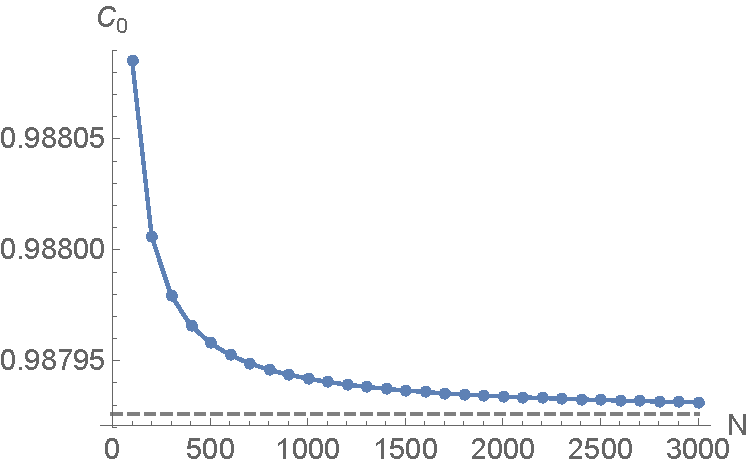
\includegraphics[scale=0.5]{quarticwfplot1.pdf}
\end{center}
%%%%%%
\section{Lowest-Energy Wavefunction for $p^4+x^4$ Hamiltonian}
Let's see if we can do a similar thing for the lowest energy wavefunction of the more conventional quartic Hamiltonian. Using David's Eq.~(9) (draft 5-24), we have
\be
H&=&-3t_1+\frac{t_1}{4}\left(\Pi_1^4+\Pi_2^4\right)\\
&=&\frac{t_1\varepsilon^2}{8}\left[a^4+\left(a^\dagger\right)^4+6\left(a^\dagger a+\frac{1}{2}\right)^2+\frac{3}{2}\right]\\
&=&\frac{t_1\varepsilon^2}{8}\left[a^4+\left(a^\dagger\right)^4+6\left(a^\dagger a^\dagger a a +2a^\dagger a+\frac{1}{4}\right)+\frac{3}{2}\right]
\ee
We again write a general wavefunction as
\be
\ket{\psi}&=&\sum_kC_k\ket{k}
\ee
so that
\be
H\ket{\psi}&=&\omega\sum_{k}C_k\bigg[\alpha_-(k)\ket{k-4}+\alpha_+(k)\ket{k+4}+3\left(2k^2+2k+1\right)\ket{k}\bigg]\\
&=&\omega\sum_{k}C_k\bigg[\alpha_-(k)\ket{k-4}+\alpha_+(k)\ket{k+4}+\eta(k)\ket{k}\bigg]\\
&\stackrel{!}{=}&E\sum_kC_k\ket{k}.
\ee
As before, we take overlaps with a few low-energy LL states:
\be
\renewcommand\arraystretch{1.5}\begin{array}{ccccc}
\bra{0}:&&\omega\bigg[C_{4}\alpha_-(4)+C_{0}\eta(0)\bigg]&=&EC_0\\
\bra{4}:&&\omega\bigg[C_{8}\alpha_-(8)+C_{0}\alpha_+(0)+C_{4}\eta(4)\bigg]&=&EC_4\\
\bra{8}:&&\omega\bigg[C_{12}\alpha_-(12)+C_{4}\alpha_+(4)+C_{8}\eta(8)\bigg]&=&EC_8\\
&&\vdots && \\
\bra{4p}:&&\omega\bigg[C_{4(p+1)}\alpha_-(4(p+1))+C_{4(p-1)}\alpha_+(4(p-1))+C_{4p}\eta(4p)\bigg]&=&EC_{4p}.
\end{array}
\ee
Numerically, the lowest energy level (with $\omega=1$) rapidly converges to
\be
E_0&\approx&2.79346\\
C^{(0)}_0&=&0.999104\\
C^{(0)}_4&=&-0.0421227\\
C^{(0)}_8&=&0.00411927\\
C^{(0)}_12&=&-0.000494123.
\ee
It doesn't seem as easy to solve it by inspection as before. Instead, let's try to find a recursion relation for general $E$ given $C_0$.
\be
C_4&=&\left(\frac{E-\eta(0)}{\alpha_-(4)}\right)C_0\\
C_8&=&\left(\frac{E-\eta(4)}{\alpha_-(8)}\right)C_4-\frac{\alpha_+(0)}{\alpha_-(8)}C_0\\
&=&\left(\frac{E-\eta(4)}{\alpha_-(8)}\right)\left(\frac{E-\eta(0)}{\alpha_-(4)}\right)C_0-\frac{\alpha_+(0)}{\alpha_-(8)}C_0\\
&=&\frac{\left(E-\eta(4)\right)\left(E-\eta(0)\right)}{\alpha_-(8)\alpha_-(4)}C_0-\frac{\alpha_+(0)}{\alpha_-(8)}C_0\\
&=&\frac{\left(E-\eta(4)\right)\left(E-\eta(0)\right)-\alpha_+(0)\alpha_-(4)}{\alpha_-(8)\alpha_-(4)}C_0\\
C_{k+4}&=&\frac{E-\eta(k)}{\alpha_-(k+4)}C_k-\frac{\alpha_+(k-4)}{\alpha_-(k+4)}C_{k-4}\\
\Rightarrow C_{k}&=&\frac{E-\eta(k-4)}{\alpha_-(k)}C_{k-4}-\frac{\alpha_+(k-8)}{\alpha_-(k)}C_{k-8}
\ee




\end{document}